\chapter{Kiosks}
\label{chapter:kiosks}

\section{Introduction}
\label{section:introduction}
This task set is concerned with building kiosks in villages and models another central graph problem in information technology. The algorithmic problem lying beneath this task is called Dominating Set Problem. For a given graph with vertices and edges, the algorithm tries to find a minimal set of vertices such that every vertex of the given graph has either the vertex itself or an adjacent vertex that is part of the selection.

In this task set, a kiosk (see figure \ref{fig:kiosk}) can be selected and then be built on a point in the graph. There are different maps containing a village network with points and interconnections (see figure \ref{fig:kioskExample}).
Throughout the levels, the user has to check given kiosk distributions and find own solutions. The challenge is to place kiosks in a way that all points of the map representing villages have close access to a kiosk. A village has close access to a kiosk if and only if it has a kiosk itself, or there is a neighbouring village with a kiosk.

\begin{figure}[H]
    \centering
    
\includegraphics[width=0.2 \columnwidth]{figures/kiosk.png}
    \caption{The Kiosk} 
    \label{fig:kiosk} 
\end{figure}

\begin{figure}[H]
    \centering
    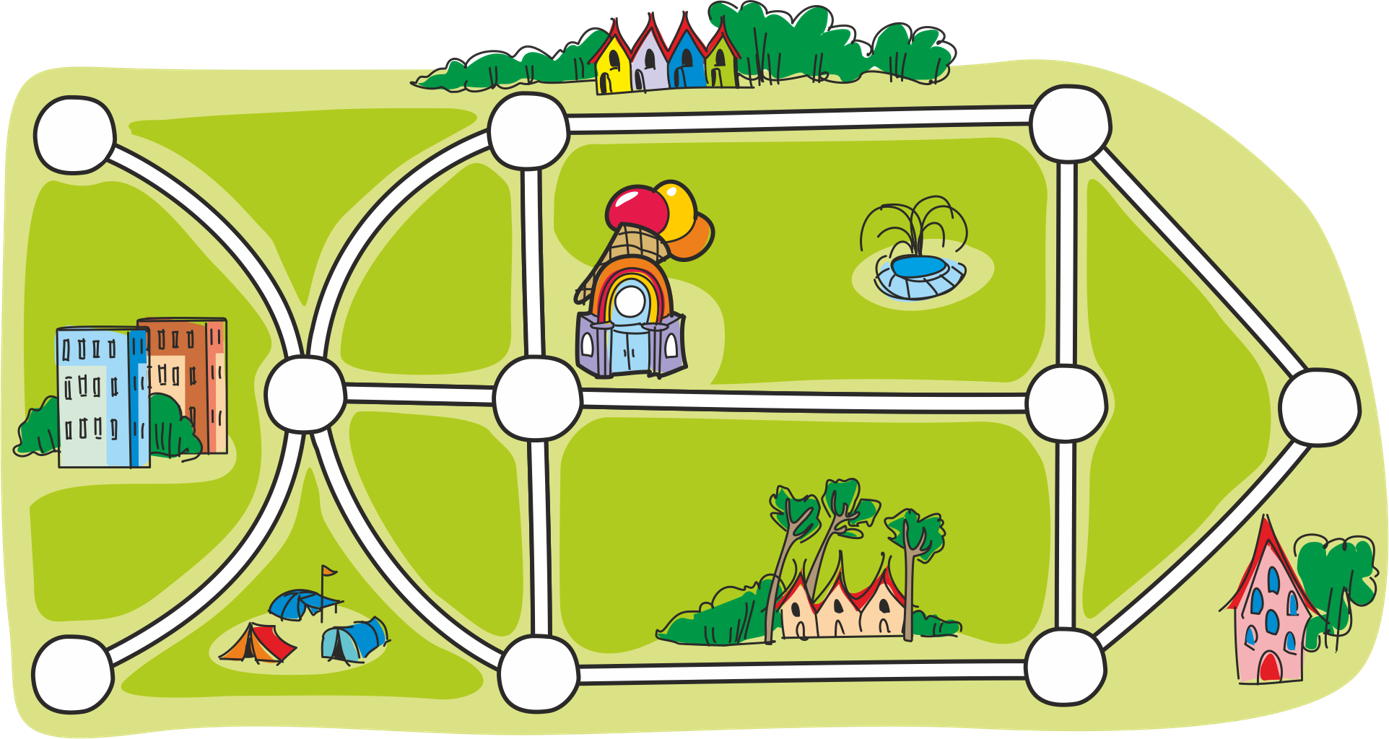
\includegraphics[width=1.0 \columnwidth]{figures/kiosk_example.png}
    \caption{Example of a Map} 
    \label{fig:kioskExample} 
\end{figure}


\section{Levels and Goals}
\label{section:assignment}

Similar to the previously discussed \nameref{chapter:towers}, the goal of this exercise is that the student finds strategies to cover a graph with as few kiosks as possible. The users are encouraged to reflect on different points in the graph where kiosks could be placed and how useful a particular place is (that is, how many villages it provides access to). 

The levels correspond to the structure of the towers exercise: On the first level, the students are required to check if the placed kiosks build a dominating set. Often, there are more villages covered with a single kiosk than the user would intuitively expect.

On the second level, the students have to build kiosks in villages, such that all villages have a kiosk close by. Again, the number of kiosks is set for each map individually. Also, the number is small enough such that kiosks cannot be placed on every single point.

On the third level, the task is to find an optimal solution. The number of kiosks for an optimal solution is not indicated.


\section{Implementation}
\label{section:implementation}
Similarly to the towers exercise, the implementation of the task levels is also based on a game template and on a map template. The game template is called Kiosks.vue and defines the main structure, design, and meta functionality. The map template called KiosksTemplate.vue then specifies the particular functions for a map that is then dynamically injected into the game template. Also, the \nameref{subsection:statementcheck} is located in Kiosks.vue.

Just as in the towers exercise, each map has an underlying graph that is modelled according to the graph drawn on the map. The graph is represented by the same graph class.

One of the main differences to the towers task set is the algorithm to test the correctness of a solution. The testing is run over every solution proposition, independent if it was created by the computer or the user. The test checks if the proposition complies with all the regulations and consists of an algorithm that checks - in contrast to the towers exercise - if the chosen vertex set forms a dominating set. As a first step, all chosen vertices (contained in the array called arr) of the underlying graph are added to a set called coveredVertices (see code below). Additionally, all neighbours of the vertex are added to the set when a vertex is checked and added to the set. If the solution is correct, the set contains every vertex of the graph after the algorithm has terminated. The verification algorithm can be seen below in a simplified version:

%TC:ignore
\begin{lstlisting}[language=TypeScript,caption={},label={lst:isDominatingSet}]
  isDominatingSet(arr:unknown[]):boolean {
    const coveredVertices = new Set();
    for (let i = 0; i < arr.length; i += 1) {
      for (const j of adjList.get(arr[i])) {
        coveredVertices.add(j);
      }
      coveredVertices.add(arr[i]);
    }

    // if every vertex has a marked neighbor, the set size corresponds to the total number of vertices
    const solution = (coveredVertices.size === numberOfVertices); // assigns a boolean value
    return solution;
  }
\end{lstlisting}
%TC:endignore

The correctness of the user input is verified just as described in the chapter on \nameref{chapter:towers}: The correctness of the level 1 proposition is immediately verified by the dominating set algorithm when a random set is generated. Whenever the verify button is clicked, all the program does is comparing the user input to the result of the aforementioned algorithm.

The second level is checked as soon as the user has finished an own proposition. A solution is permissible if and only if the user has chosen a dominating set.

In the optimization task, not only the implemented dominating set check is run, as in level 2, but the proposition is also tested if it is optimal. To do so, the algorithm simply compares the number of used kiosks to the number of kiosks used in the optimal solution. Whenever both checks are evaluated positively, the result is emitted and said to be true.